\iffalse
\documentclass[journal,12pt,twocolumn]{IEEEtran}
\usepackage{amsmath,amssymb,amsfonts,amsthm}
\usepackage{txfonts}
\usepackage{tkz-euclide}
\usepackage{listings}
\usepackage{gvv}
\usepackage[latin1]{inputenc}
\usepackage{array}
\usepackage{pgf}
\usepackage{lmodern}

\begin{document}
\bibliographystyle{IEEEtran}

\vspace{3cm}

\title{}
\author{EE23BTECH11054 -  Sai Krishna Shanigarapu$^{*}$
}
\maketitle
\newpage
\bigskip



\section*{Exercise 9.2}

13. \hspace{2pt}If the sum of $n$ terms of an A.P. is $3n^2+5n$ and its $m^{th}$ term is 164, find the value of $m$.
\bigskip

\solution
\fi
\begin{align}
Y\brak{z} &=  \sum_{n=0}^{\infty} y\brak{n}z^{-n} \\
&= \frac{2\brak{4-z^{-1}}}{\brak{1-z^{-1}}^3}, \qquad |z| > 1\\
U\brak{z} &= \frac{1}{1-z^{-1}}, \qquad |z| > 1\\
X\brak{z} &=  \frac{Y\brak{z}}{U\brak{z}}\\
 &= 2\brak{\frac{1}{1-z^{-1}}} + 6\brak{\frac{1}{\brak{1-z^{-1}}^2} } \\
 &= \frac{8z^2 - 2z}{\brak{z-1}^2} 
\end{align}


Using Contour Integration to find the inverse Z-transform,
\begin{align}
   x\brak{n} &= \frac{1}{2\pi j}\oint_C X\brak{z}z^{n-1}dz\\
    &= \frac{1}{2\pi j}\oint_C \frac{\brak{8z^{n+1} - 2z^{n}}dz}{\brak{z-1}^2}\\
    &= \frac{1}{\brak{m-1}!}\lim_{z\to\ a}\frac{d^{m-1}}{dz^{m-1}}\brak{\brak{z-a}^m f\brak{z}}\\
    &= \lim_{z\to\ 1}\frac{d}{dz}\brak{\brak{z-1}^2 \frac{8z^{n+1} - 2z^n}{\brak{z-1}^2}}\\
    &= \lim_{z\to 1}\brak{8\brak{n+1}z^n - 2nz^{n-1}}\\
    \implies x\brak{n} &= \brak{6n+8}\brak{u\brak{n}}\\
    164 &= \brak{6m+8}\brak{u\brak{m}}\\
    \implies m &= 26
\end{align}

\setlength{\arrayrulewidth}{0.3mm}
\setlength{\tabcolsep}{15pt}
\renewcommand{\arraystretch}{1.4}

\begin{table}[ht]
\centering

\begin{tabular}{|c|c|}
\hline

Symbol & Remarks\\
\hline
$y\brak{n} =\brak{3n^2+11n+8}\brak{u\brak{n}}$ & Sum of $n$ terms  \\
\hline
$x(m-1)$ & $164$\\
\hline
$y\brak{n}$ & $x\brak{n} * u\brak{n}$\\
\hline

\end{tabular}
\vspace{0.25cm}
\caption{Parameters}
\label{tab:11.9.2.13.1}



\end{table}



\begin{figure}[htbp]
    \centering
    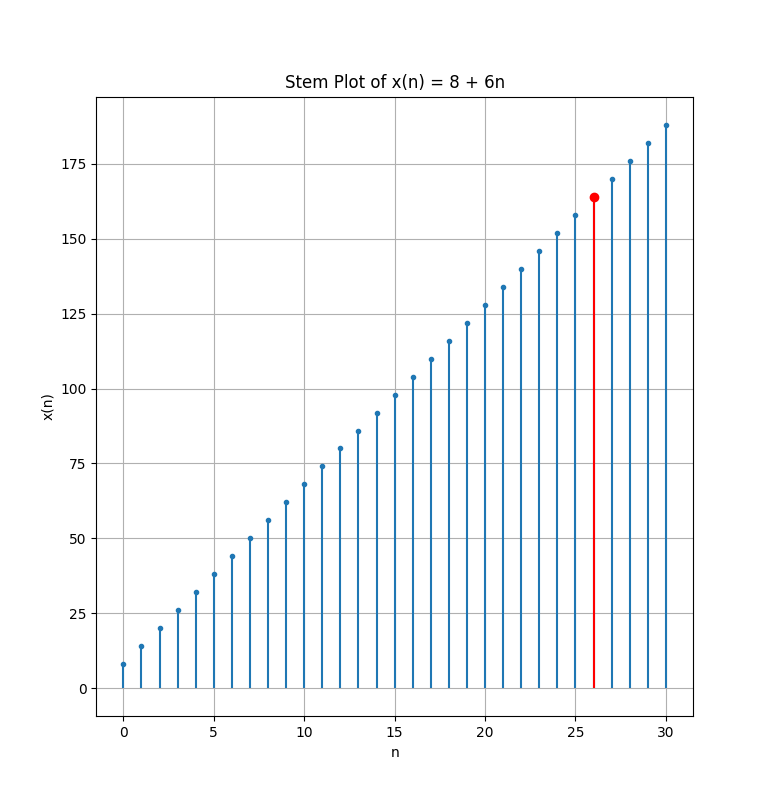
\includegraphics[width=1.0\columnwidth]{ncert-maths/11/9/2/13/figs/Figure_1.png}
    \caption{Plot of x(n) vs n}
    \label{fig:11.9.2.13.1}
\end{figure}


%\end{document}
